\subsection{Program individual registers of slave GBTx}
\label{sec:software-slave-individual}
Before proceed, follow \autoref{sec:hardware-slave-sca} to set up hardware.
Again we use \textbf{GBT Client} to program individual registers of the slave
GBTx.
Configure the parameter \emph{exactly} as shown in \autoref{fig:gbt-i2c}.

\begin{figure}[ht]
    \centering
    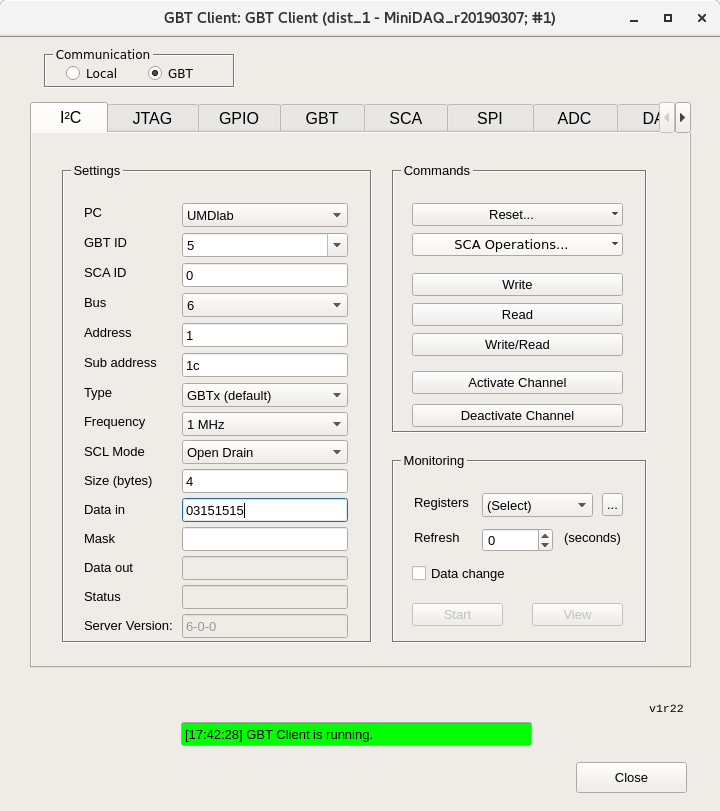
\includegraphics[width=0.9\textwidth]{res/gbt_client_slave_gbt_i2c_test.png}
    \caption{Correct parameters to configure GBT \itwoc tab.}
    \label{fig:gbt-i2c}
\end{figure}

\begin{leftbar}
    If the \textbf{Write} command failed, try \textbf{Activate Channel} first.
\end{leftbar}

\begin{leftbar}
    \textbf{Address} corresponds to GBTx index, which is configured via an
    onboard DIP switch. Default to 1.
\end{leftbar}

\begin{leftbar}
    Recall that 1 \emph{Byte} is 8 \emph{bits}, and 1 Byte corresponds to a
    2-digit hex number.
\end{leftbar}

\begin{leftbar}
    Notice in the \textbf{Data out} field, the last 3 numbers are the same.
    This is a requirement in the GBT specification that the configuration
    registers must be triplicated to minimize error.
\end{leftbar}
